\documentclass[a4paper]{article}
\usepackage[T1]{fontenc}
\usepackage[utf8]{inputenc}
\usepackage{lmodern}
\usepackage{graphicx}
\usepackage[left=2.5cm,right=2.5cm,top=3cm,bottom=3cm]{geometry}
\usepackage{eurosym}
\usepackage{fancyhdr}%encabezado y pie de página
\usepackage[colorlinks=true, linkcolor=black, urlcolor=blue]{hyperref}
\setcounter{secnumdepth}{5}
\usepackage[spanish]{babel}
\setcounter{tocdepth}{5}
\usepackage{colortbl}%para colorear tablas
\usepackage{tabularx}
\usepackage{placeins}%para poner barrera y no pasen de secciones los elemntos flotantes
%\usepackage{wasysym} %para poner símbolos
\usepackage{bbding} %para poner símbolos



%para el mapa mental
\usepackage{tikz}
\usetikzlibrary{mindmap,trees}
\usepackage{verbatim}


\date{}
\author{D. Ramirez Ambrosi \\ J. I. Sánchez Méndez \\ J. Rodríguez Azpeleta}
\title{\begin{center}
\textbf{\Huge{Make Yourself Strong}} \\ Análisis de necesidades  \\Proyecto de la asignatura Interacción Persona Computador \\ \Huge{Grupo 10}
\end{center}}
\date{\today}


\pagestyle{fancy}
\rhead{
\textbf{Make Yourself Strong} \hfill \textbf{Fecha:} \date{\today}
}

\lhead{}

%Separación entre párrafos
\setlength{\parskip}{3mm}

%colores
\definecolor{verde}{RGB}{127,255,0}%color para la barra de titulo
\definecolor{rojo}{RGB}{255,0,0}%color para características
\renewcommand\listfigurename{\centering LISTA DE FIGURAS}

\begin{document}
\maketitle

\thispagestyle{empty}%para evitar enumeración de la página de la portada y del índice
\newpage
\tableofcontents%índice
\thispagestyle{empty}
\newpage



%lista de figuras 
%\renewcommand\listfigurename{\centering LISTA DE FIGURAS}
%\listoffigures
%\clearpage

%Lista de tablas
%\renewcommand{\listtablename}{\centering ÍNDICE DE TABLAS} %Para cambiar el índice de las tablas
%\listoftables
%\thispagestyle{empty}
%\newpage

\setcounter{page}{1}%Para reinizar el contador de páginas en la página deseada


\section{Introducción}

La prueba está basada en el uso de la aplicación \textbf{MyFitnessPAL} \footnote{\url{http://www.myfitnesspal.com.mx}}. Esta aplicación está centrada en la cuenta de calorías de un usuario. En base a parámetros - como la altura, peso y nivel de actividad física - y objetivos - como mantener o variar el peso - muestra una estimación de las calorías que el usuario debe consumir al día así como la cantidad de macronutrientes (hidratos de carbono, grasas y proteínas) que debe consumir para alcanzar los objetivos deseados.

Los usuarios pueden realizar el seguimiento calórico mediante el registro de los alimentos consumidos mediante búsquedas en la base de datos propia. También tienen la posibilidad de añadir un alimento en caso de no encontrarlo en dicha base de datos.

También tienen la posibilidad de registrar las calorías consumidas por ejercio físico. Como en el caso anterior, se puede buscar el ejercicio en la base de datos o añadirlo en caso de que no se encuentre.

Los usuarios pueden realizar su propio seguimiento mediante la consulta de estadísticas gráficas.

\section{Observación de participantes}

	\subsection{Jonathan Castro}
	
	Estudiante de Ingeniería informática, práctica deporte de forma regular.
	
		\subsubsection*{Registro de usuario}
		
		Llevado a cabo sin mayores dificultades. Resultó molesto que se pidiera información como la fecha exacta de nacimiento - Con el año para el cálculo de la edad serviría - así como el código postal y ciudad de residencia.
		
		Durante el registro se pregunta sobre los objetivos, las descripciones del nivel de actividad no resultan muy descriptivas. Además, no determinan de forma clara si en ese nivel de actividad se incluye el que se haga ejercicio regularmente o únicamente trata el nivel de actividad habitual referente a la profesión de la persona.
		
		\subsubsection*{Añadir un entrenamiento}
		
		Tras añadir un entrenamiento, se muestra en una tabla. Se da la opción de eliminarlo, aunque no se ve claramernte está función ya que viene representada por un icono con una señal de prohibición. Un icono más representativo de la función eliminar evitaría confusiones.
		
		En el caso de añadir un entrenamiento de fuerza, solo se puede añadir para un entrenamiento determinado un número de series con el mismo peso y repeticiones para cada una de las mismas. En este caso se hubiera querido especificar el peso y repeticiones para cada serie concreta.
		
		Al contabilizar las calorías quemadas en el entrenamiento, se muestran solo las correspondientes al entrenamiento cardiovascular y no se tienen en cuenta las del entrenamiento de fuerza.
		
		Otro defecto fue que las estimaciones de las calorías no eran exactas en determinados entrenamientos.
		
		Una sugerencia en este apartado fue que se tuvieran en cuenta patologías que el usuario pudiera tener para que la aplicación pudiera indicar si se daban casos de sobreesfuerzo.
		
		\subsubsection*{Añadir alimentos}
		
		En general, ningún defecto en cuanto a la interacción. El problema viene de la estimación dada para algunos alimentos
		
		\subsubsection*{Comentarios y mejoras generales}
		
		Estimaciones, tanto en calorías de los entrenamientos, como de macronutrientes de los alimentos y estimación de objetivos.
		
		En cuanto a menús, los botones de sesión, menos destacados que el resto, quedan poco a la vista. El calendario para selección de fechas está en formato inglés, siendo domingo el día que se encuentra en primer lugar.
		
			\begin{figure}[!h]
				\centering
				
\includegraphics[width=0.7\textwidth]{./figuras/jonat-1.jpg}
				\caption{Jonathan navegando por la aplicación}
			\end{figure} 
		
			\begin{figure}[!h]
				\centering
				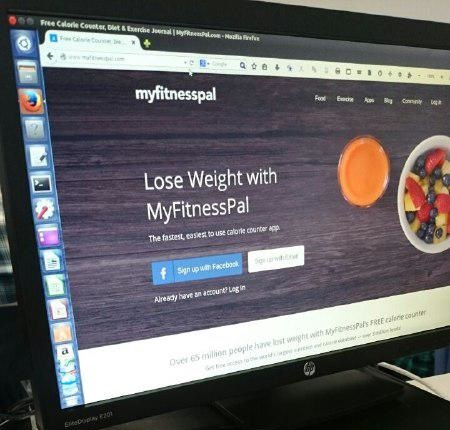
\includegraphics[width=0.5\textwidth]{./figuras/jonat-2.jpg}
				\caption{Página principal}
			\end{figure} 
			
			\begin{figure}[!h]
				\centering
				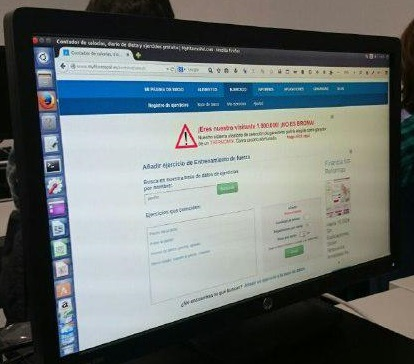
\includegraphics[width=0.5\textwidth]{./figuras/jonat-3.jpg}
				\caption{Añadiendo un ejercicio de fuerza}
			\end{figure}
		
		\FloatBarrier
		
		\subsection{Marta Aguilera}
		
		Trabaja actualmente como desarrolladora de software.
		
			\subsubsection*{Registro de usuario}
			
			Algunos datos de los requeridos por la aplicación, como el código postal y la fecha exacta de nacimiento, deberían ser opcionales. En cuanto a la fecha de nacimiento, con saber el año para calcular edad sería más que suficiente como parámetro para la aplicación.
			
			El vocabulario usado para preguntar sobre la frecuencia con que se va a practicar ejercicio resulta poco conciso. La aplicación pregunta por el número de "rutinas por semana". Ha sido necesario aclarar que se trata de días por semana que se va a practicar ejercicio, ya que rutina se asocia a una serie de ejercicios que se practican en una sesión de entrenamiento y que esta misma rutina se puede repetir varios días.
			
			En cuanto a la función de invitar a amigos, no le resulta demasiado llamativa. Si que aprecia el mensaje en que la página asegura la privacidad del peso registrado y que éste no será visible a otros usuarios.
			
			En la siguiente pantalla de objetivo los números están muy bien, pero se hechan en falta explicaciones o consejos como ``evita comer determinado tipo de alimentos''.
			
			\subsubsection*{Añadir un entrenamiento}
			
			La búsqueda de ejercicios debe ser realizada por el nombre específico del mismo. Por ejemplo, al buscar ``cinta'', no muestra ningún resultado. En su lugar hay que buscar ``correr'' donde uno de los resultados indica ``correr en el sitio'' que sería el correspondiente a usar la cinta de correr. En este sentido, la búsqueda de ejercicio debería ser "más abierta" permitiendo búsquedas por máquinas concretas o nombres más coloquiales que se pudieran al ejercicio en cuestión. Esto permitiría que la búsqueda fuera más intuitiva y no frustrante como ha resultado ligeramente para Marta.
			
			A destacar de forma positiva que los ejercicios seleccionados de forma reciente estén disponibles (bajo la barra de búsqueda) para seleccionarlos directamente sin necesidad de buscarlos de nuevo.
			
			En la pantalla general del entrenamiento destaca la función de ``herramientas rápidas'' que permiten copiar la lista de ejercicios desde una fecha concreta o copiar la lista del día actual a una fecha concreta. En cambio, el icono destinado a simbolizar la función de eliminar un entrenamiento de la lista no resulta representativo, ya que se trata de una señal de prohibición.
			
			Las listas de ``Cardiovascular'' y ``Fuerza'' están demasiado separadas entre ellas, además no se contabilizan las calorías quemadas en el entrenamiento de fuerza.
			
			Resulta de gran utilidad la función de ``Ver el informe completo (para imprimir)'' que permite ver el resumen del entrenamiento. En el se puede seleccionar un intervalo de fechas para las cuales se quiera practicar el entrenamiento creado. Está funcionalidad resultaría más útil antes, ya que permitiría aplicar el entrenamiento creado en los días deseados y sería más rápido que la opción de copiar a una fecha concreta que se ha visto antes. Un elemento que se hecha en falta en esta página de informe en un botón de vuelta atrás o de ``Terminado''.
			
			\subsubsection*{Añadir alimentos}
			
			Traducción incorrecta a diferentes idiomas, por ejemplo al añadir café, la cantidad se especificaba en número de ``cups''. En la búsqueda de alimentos resulta muy útil la posibilidad de hacer una búsqueda abierta como ``café'' y que se muestren varias opciones para seleccionar una concreta (un tipo de café determinado, una marca concreta...). Éste es el tipo de búsqueda que se hechaba en falta a la hora de buscar los entrenamientos. Además se aprecia que la cantidad de entradas de alimentos es muy grande, hay gran cantidad de datos en la base de datos de la aplicación.
			
			Otro aspecto positivo es que la misma alicación te avisa si sobrepasas los objetivos de algún elemento como las calorías, los azúcares, grasas... y también muestra mensajes gratificantes como "Si todos los días fueran como hoy, pesarías X en 5 semanas".
			
			En cuanto al agua consumida, sería mejor añadirla por comida en vez de globalmente la consumida en el día. Además, resulta poco gráfico la entrada de agua con el icono del vaso.
			
			
		\FloatBarrier
		
		\subsection{Andoni Martín}
		
			Estudiante de ingeniería informática y aficionado al trabajo hortelano.
		
			\subsubsection*{Registro de usuario}
			
			En el registro está marcada por defecto la casilla para que la aplicación envíe automáticacmente boletines al correo, no resultaría molesto si la casilla estuviera desactivada por defecto. Además, no pide confirmación de la contraseña, es decir, no hay que escribirla dos veces para comprobar que se ha escrito correctamente. Esto podría hacer que el usuario no pudiera autenticarse en el sistema tras acabar el registro y tuviera que solicitar la recuperación o cambio de la contraseña.
			
			En cuanto a datos personales se repite la opinión de que pedir la fecha de nacimiento completa no resulta necesario (el año serviría) y que este dato junto con el código postal deberían ser opcionales.
			
			A la hora de indicar la cantidad de veces que se practica deporte ha sido necesario explicar que ``rutina'' en ese caso se refería a los días a la semana que se realizará actividad física. El lenguaje utilizado no es específico y aclaratorio.
			
			En cuanto a la pantalla de selección de objetivos, se debe especificar el peso actual y el deseado, pero posteriormente pregunta cuál es tu objetivo entre opciones de ``bajar X kilos a la semana'', ``mantener'' o ``subir X a la semana''. El problema radica en que puedes indicar bajar 10 kilos de peso al especificar el peso actual y el objetivo, y luego seleccionar como objetivo aumentar peso. No resulta lógica tal selección, es probable que a un usuario no se le ocurra realizar tal selección, pero la aplicación debería avisar de esta incongruencia en caso de que se diera.
			
			El resumen de objetivos que se muestra al finalizar el registro resulta útil.
			
			\subsubsection*{Añadir un entrenamiento}
			
			En la pantalla se hace la distinción entre entrenamiento ``cardiovascular'' y ``de fuerza'', Andoni sabía a qué se refería cada uno, pero otros usuario pueden necesitar de ayuda, una explicación en pantalla de cuál es la diferencia entre ambos y por qué están separados.
			
			A la hora de añadir un entrenamiento de tipo cardiovascular, se pregunta por el tiempo de duración de dicho ejercicio, pero no se especifican las unidades en que se mide el tiempo. En cuanto a la búsqueda, le gusta que aparezca ``pasear al perro'' y que conduzca a una única opción, aunque, en general, la búsqueda de ejercicios debe hacerse de forma específica con el nombre técnico del entrenamiento.
			
			Además de añadir los diferentes ejercicios al entrenamiento, también se permiten añadir notas sobre el mismo. Resulta molesto que no se pueda escribir directamente en el campo de texto, que sería lo más directo, y que haya que pulsar en un pequeño botón de editar.
			
			Otra cosa que resulta un tanto molesta es que el entrenamiento se guarde automáticamente a cada ejercicio que se introduce. En su lugar, estaría mejor un botón de ``Aceptar'' o ``Guardar entrenamiento'' y que el botón de ``Imprprimir entrenamiento'' apareciera como secundario del formulario y no como único que es el caso actual.
			
			\subsubsection*{Añadir alimentos}
			
			\subsubsection*{Comentarios y mejoras generales}
			
			En cuanto al diseño de la página, las acciones en algunos sitios se presentan como botones (en la página principal por ejemplo) y en otros casos como enlaces (en las ventanas de entrenamiento o alimentación, las funciones de añadir entrenamientos o alimentos respectivamente).
			
			En la pantalla principal no resultan claros los nombres de las funcionalidades dados en los botones. ``Añadir alimento'' enlaza con la página para añadir los alimentos de un día, pero ``Añadir'' a secas enlaza con añadir un entrenamiento. Debería ser ``añadir entrenamiento'' que especifica qué es lo que se va a añadir en ese botón.
			
			En esta pantalla se muestra también una barra que indica los días seguidos que se ha hecho el seguimiento de la actividad física. Su diseño induce a pensar que se trata de un elemento deslizable que el usuario puede ajustar.
			
		\FloatBarrier
		

\section{Necesidades identificadas}

A continuación se detallan las diferentes necesidades detectadas en las diferentes observaciones.

	\subsection{Descripciones de elementos}
	
	Las descripciones que se asocien a diferentes elementos de una lista de opciones tienen que ser lo suficientemente claras para que el usuario no tenga ninguna duda de cuál es la que le conviene marcar.
	
	Este problema se da en el caso de la selección de la actividad diaria realizada donde se ejemplifica cada opción con una profesión pero no queda claro si se incluye la actividad física no asociada a la profesión que la persona pueda realizar.
	
	\subsection{Estimaciones más exactas}
	
	En general, ya sea al estimar los objetivos del usuario, las calorías y macronutrientes asociados a un alimento o las calorías consumidas por un determinado ejercicio, procurar, en la medida de lo posible, ofrecer valores más exactos al usuario.
	
	\subsection{Localización del usuario}
	
	En el caso del calendario, su formato era inglés. De cara a ofrecer un mejor servicio, se debería adaptar el calendario o incluso las unidades de medida al sistema utilizado en el lugar desde el que el usuario realiza la conexión.
	
	\subsection{Iconos representativos}
	
	En el caso de funciones básicas como eliminar un elemento, añadirlo o modificarlo, no se puede dar lugar a dudas de la acción representada por el icono en cuestión.
	
	\subsection{Registro de entrenamientos más preciso}
	
	Permitir especificar para un ejercicio de fuerza las diferentes series de forma individual, con un peso y repeticiones concretos para cada serie.
	
	\subsection{Registro de patologías}
	
	Permitir al usuario problemas que padezca (asma, problemas de corazón, dañoos musculares...), de forma que la aplicación avise en caso de sobre esfuerzo en base a los ejercicios añadidos a un entrenamiento.
	
	\subsection{Destacar los botones de sesión}
	
	Hacer que sean perfectamente visibles para que el usuario encuentre fácilmente, por ejemplo, el cierre de sesión.



\end{document}